\documentclass[a4paper,12pt]{article}

% don't forget the document class, generally : \documentclass[a4paper,12pt]{article}

\usepackage[utf8]{inputenc}
\usepackage[french]{babel}
\usepackage{graphicx}
\usepackage{gensymb}
\usepackage{amsmath}
\usepackage{float}
\usepackage{scrextend}
\usepackage{caption} 
\usepackage{siunitx}
\usepackage{enumitem}
\usepackage{amsthm}
\usepackage{fancyhdr}
\usepackage{amssymb}
\usepackage{wrapfig}
\usepackage{geometry}
\usepackage{standalone}
\usepackage{import}
\usepackage[usenames, dvipsnames]{color}

 \usepackage{biblatex} % manages bibliography and references
\addbibresource{sample.bib}


\geometry{hmargin=1in, vmargin=1in}

 \newenvironment{absolutelynopagebreak}
 {\par\nobreak\vfil\penalty0\vfilneg
 \vtop\bgroup}
 {\par\xdef\tpd{\the\prevdepth}\egroup
 \prevdepth=\tpd}
 
 \pagestyle{fancy}                        
\fancyhf{}                               
\fancyhf[HL]{Application des maths}                
\fancyhf[HR]{Géométrie euclidienne}             
\fancyhf[FC]{\thepage/\pageref{Lastpage}}
 
\newtheorem{definition}{Définition}[section]
\newtheorem{theorem}{Théorème}
\newtheorem{corollary}{Corollaire}[theorem]
\newtheorem{lemma}[theorem]{Lemme}
\newtheorem*{hyp}{Hypothèse}
\newtheorem*{concl}{Conclusion}
\newtheorem*{remark}{Remarque}

\captionsetup{format=default,labelformat=simple,labelsep=colon,
justification=justified,font={sf,small},labelfont=bf,
textfont=default} 



\begin{document}

\section{Courte biographie d'Euclide}

\begin{figure}[H]
    \centering
    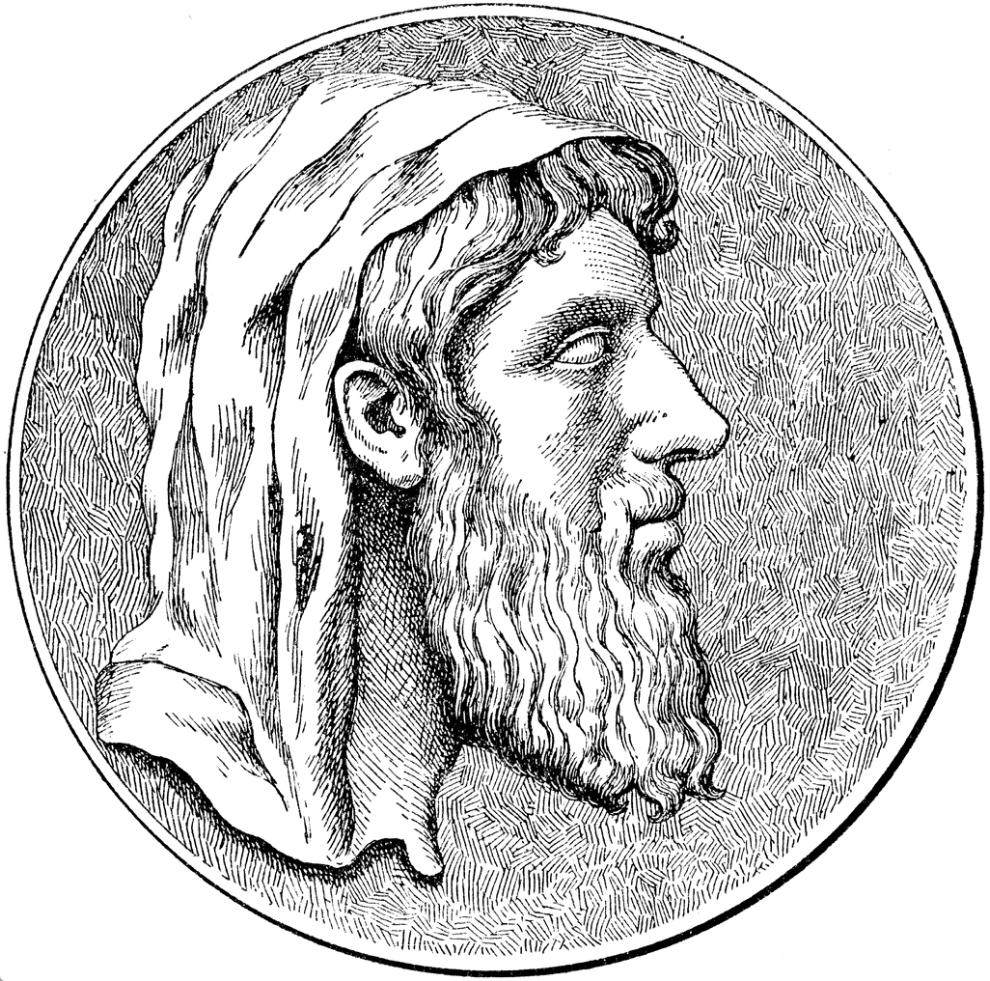
\includegraphics[scale=0.2]{schema/portrait.png}
\end{figure}
Euclide est un mathématicien grec ayant vécu aux alentours de 300 avant J.C.. Il n'y a que très peu d'information à son sujet si ce n'est qu'il a enseigné au musée d'Alexandrie sous Ptolémée $1^{er}$. Euclide ne fut sûrement pas le premier à s'être intéressé à la géométrie, mais la raison pour laquelle on l'appelle le père de la géométrie est "Les éléments d'Euclide". Cet écrit mathématique et géométrique est constitué de treize volumes, qui traitent des fondements de la géométrie euclidienne: des axiomes aux théorèmes et leurs démonstrations. Grâce à la simplicité et la logique de ce recueil, il a été utilisé comme livre de référence durant des siècles.

\end{document}